%% smpost/thumbnail/chapter_10_crowd_at_the_border.tex : thumbnail of video 10/30,
%% "Chapter-10 | The Footprints at the Crossings: The Simulated RAW Hits". Motif:
%% the barrel of CMS seen along the beam, as on the thumbnail of chapter 9, but
%% now everybody moves. The charged members of the family bend in the field and
%% leave a yellow hit on every layer of silicon they cross; one of them is a
%% looper and never gets out; a photon flies straight. Showers light up the
%% crystals (green ring) and the scintillator (orange ring); the iron stays
%% dark. The grey dots on the layers are the footprints of the crowd.
%% Compile: make thumbnails-youtube   (or: pdflatex chapter_10_crowd_at_the_border)
\documentclass[tikz,border=0pt]{standalone}
%% ==========================================================================
%% smpost/thumbnail/thumbnail_common.tex : what every JitJet video thumbnail
%% shares. Each chapter_XX_*.tex in this directory is a standalone TikZ
%% document that \input{}s this file after \documentclass and then draws its
%% own motif on the right of the page.
%%
%% The page is 19.2 cm x 10.8 cm, i.e. 1280 x 720 px at 1 px = 0.015 cm, the
%% YouTube thumbnail size (16:9). `make thumbnails-youtube` compiles every
%% chapter_*.tex here and rasterises it with gs to a 1280 x 720 PNG.
%%
%% Layout: the wordmark top left, the "n / 30" pill top right, the stop number
%% in a milestone ring with the chapter label, the title in two big lines and
%% the subtitle under it, all in the left 10 cm; the motif of the chapter sits
%% in the right part, centred on (\mx, \my), inside about 8 cm x 8 cm, over a
%% soft gold glow.
%%   \thumbbackground
%%   \thumbtext{<stop number>}{<chapter label>}{<n / 30>}{<title, with \\>}{<subtitle>}
%% ==========================================================================
\usepackage[T1]{fontenc}
\usepackage{lmodern}
\usepackage{tgheros}          % TeX Gyre Heros, as on the cover
\usepackage{amssymb}
\usetikzlibrary{calc,arrows.meta,decorations.pathmorphing,decorations.markings,shapes.geometric}
\hyphenpenalty=10000 \exhyphenpenalty=10000   % no hyphens in titles and subtitles

%% -------- palette (identical to cover.tex) ----------------------------------
\definecolor{navy}{HTML}{0B1D3A}
\definecolor{navytop}{HTML}{17365F}
\definecolor{gold}{HTML}{F4B942}
\definecolor{bred}{HTML}{FF5A5A}     % b quark
\definecolor{bblue}{HTML}{6E8EFF}    % bbar
\definecolor{fsr}{HTML}{3DD16E}      % FSR gluons
\definecolor{isr}{HTML}{FF9A3C}      % ISR gluon
\definecolor{hadroncol}{HTML}{FFC24D}
\definecolor{ecalcol}{HTML}{3FBF77}
\definecolor{hcalcol}{HTML}{E58F2A}
\definecolor{steel}{HTML}{9AA7B8}
\definecolor{trackcol}{HTML}{E4ECF7}
\definecolor{pu}{HTML}{8D9AAB}
\definecolor{nucol}{HTML}{5EE7EA}
\definecolor{muoncol}{HTML}{8FB8FF}

%% -------- the cone of the cover, for thumbnails that show it ----------------
\def\kk{0.30}
\pgfmathdeclarefunction{rf}{1}{\pgfmathparse{0.18*#1+0.6*(1+((#1-16.8)/1.2)/sqrt(1+((#1-16.8)/1.2)^2))}}
\pgfmathdeclarefunction{sc}{1}{\pgfmathparse{min(rf(#1)/2.2,1)}}
\newcommand{\xy}[3]{({#1+\kk*#2*sc(#1)*cos(#3)},{#2*sc(#1)*sin(#3)})}
\newcommand{\xring}[2]{%
  \draw[ringback] ({#1},{#2}) arc[start angle=90, end angle=-90, x radius={\kk*#2}, y radius={#2}];
  \draw[ring]     ({#1},{#2}) arc[start angle=90, end angle=270, x radius={\kk*#2}, y radius={#2}];}
\newcommand{\xellipse}[3][]{\path[#1] ({#2},0) ellipse [x radius={\kk*#3}, y radius={#3}];}

%% -------- where the motif goes ----------------------------------------------
\def\mx{14.6}
\def\my{5.3}

%% -------- styles ------------------------------------------------------------
\tikzset{
  ring/.style={draw=gold!75!white, line width=0.6pt, opacity=0.9},
  ringback/.style={draw=white, line width=0.4pt, opacity=0.3, dash pattern=on 1pt off 1pt},
  meridian/.style={draw=white, line width=0.3pt, opacity=0.15},
  edge/.style={draw=gold!80!white, line width=1.1pt},
  bline/.style={draw=bred, line width=3pt, line cap=round},
  bbarline/.style={draw=bblue, line width=3pt, line cap=round},
  qline/.style={draw=trackcol, line width=2pt, line cap=round},
  gluon/.style={draw=fsr, line width=1.6pt, decorate,
    decoration={coil, aspect=0.6, segment length=4pt, amplitude=2.6pt}},
  isrgluon/.style={gluon, draw=isr},
  quark/.style={draw=hadroncol, line width=1.6pt, line cap=round},
  string/.style={draw=hadroncol, line width=2.4pt, line cap=round},
  hadron/.style={circle, fill=hadroncol, draw=navy, line width=0.6pt, inner sep=0pt, minimum size=9pt},
  track/.style={draw=trackcol, line width=1.3pt, line cap=round},
  pudot/.style={circle, fill=pu, inner sep=0pt, minimum size=4pt, opacity=0.8},
  pf/.style={circle, inner sep=0pt, minimum size=5pt, draw=navy, line width=0.3pt},
  roadline/.style={draw=gold, line width=1.4pt, dash pattern=on 7pt off 5pt},
  milestone/.style={circle, draw=gold, fill=navy, line width=1.6pt, minimum size=26pt,
    inner sep=0pt, font=\sffamily\bfseries\large, text=gold},
  mlabel/.style={font=\sffamily\bfseries, text=white, align=center, inner sep=4pt,
    fill=navy, rounded corners=2pt, draw=gold, line width=0.8pt},
  flight/.style={draw=bred, line width=1.4pt, dash pattern=on 4pt off 3pt},
  vertex/.style={circle, draw=bred, fill=navy, line width=1.6pt, inner sep=0pt, minimum size=9pt},
  arrowg/.style={-{Stealth[length=7pt]}, draw=gold, line width=1.2pt},
  motiflabel/.style={font=\sffamily\bfseries\small, inner sep=1.5pt},
}

%% -------- the page ----------------------------------------------------------
\newcommand{\thumbbackground}{%
  \useasboundingbox (0,0) rectangle (19.2,10.8);
  \clip (0,0) rectangle (19.2,10.8);
  \shade[top color=navytop, bottom color=navy!80!black] (0,0) rectangle (19.2,10.8);
  \draw[white, opacity=0.045, line width=0.3pt, step=1cm] (0,0) grid (19.2,10.8);
  \shade[inner color=gold, outer color=navy, opacity=0.16] (\mx,\my) circle[radius=4.6];
  \draw[gold, line width=0.6pt, opacity=0.8] (0.9,0.85) -- (18.3,0.85);
  \node[anchor=south west, gold!80!white, font=\sffamily\scriptsize] at (0.9,0.95) {Journey Is The Jet \,$\cdot$\, bottom to top};
  \node[anchor=south east, white!70!navy, font=\sffamily\scriptsize] at (18.3,0.95) {github.com/ravindkv/JitJet};
}

%% \thumbtext{stop}{chapter label}{n / 30}{title}{subtitle}
\newcommand{\thumbtext}[5]{%
  \node[anchor=west] at (0.9,9.65)
    {\fontsize{26}{28}\selectfont\sffamily\bfseries{\color{white}Jit}{\color{gold}Jet}};
  \node[anchor=east, gold, font=\sffamily\bfseries\small, draw=gold, line width=0.8pt,
        rounded corners=6pt, inner xsep=7pt, inner ysep=3.5pt] at (18.3,9.65) {#3};
  \node[milestone] (stop) at (1.45,7.85) {#1};
  \node[anchor=west, gold, font=\fontsize{15}{17}\selectfont\sffamily\scshape] at (2.1,7.85) {#2};
  \node[anchor=north west, white, align=left, inner sep=0pt,
        font=\fontsize{34}{39}\selectfont\sffamily\bfseries] (ttl) at (0.9,7.05) {#4};
  \node[anchor=north west, gold!90!white, align=left, inner sep=0pt, text width=9.6cm,
        font=\fontsize{14}{17}\selectfont\sffamily\itshape] at ($(ttl.south west)+(0,-0.4)$) {#5};
}

\begin{document}
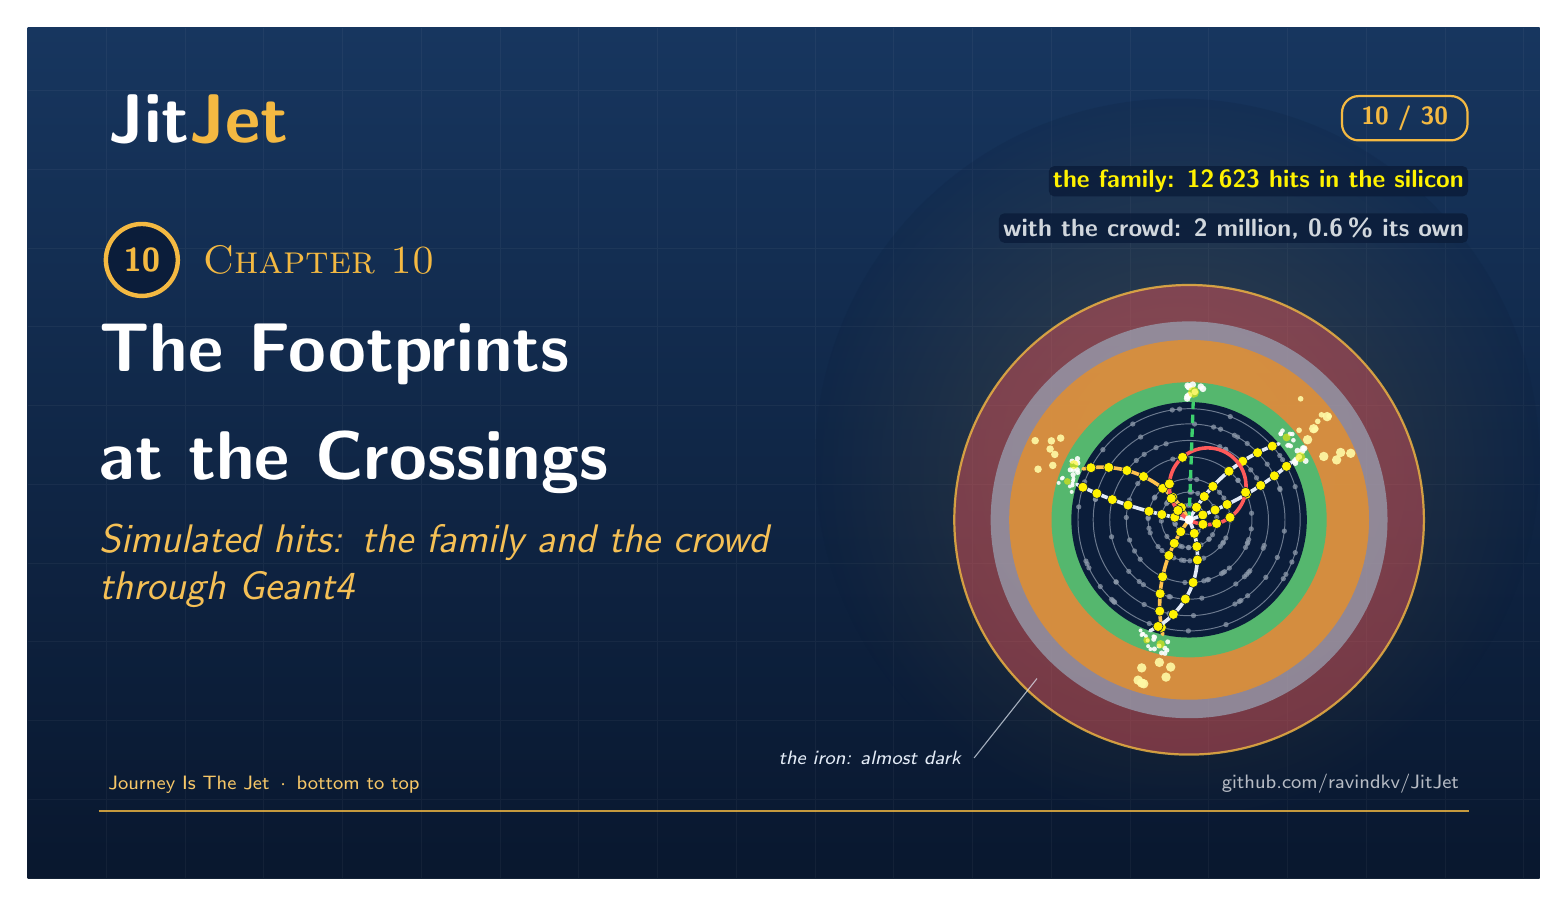
\begin{tikzpicture}[x=1cm,y=1cm]
\thumbbackground
\thumbtext{10}{Chapter 10}{10 / 30}{The Footprints\\at the Crossings}{Simulated hits: the family and the crowd through Geant4}

\begin{scope}[shift={(\mx+0.15,\my-0.75)}, scale=0.84]
%% the detector: iron, coil, HCAL, ECAL, the tracker volume
\foreach \r/\c/\o in {3.55/bred/0.42, 3.0/steel/0.7, 2.72/hcalcol/0.8, 2.08/ecalcol/0.85}
  \fill[\c, opacity=\o] (0,0) circle[radius=\r];
\fill[navy] (0,0) circle[radius=1.78];
\draw[gold, line width=0.8pt, opacity=0.8] (0,0) circle[radius=3.55];
%% the layers of silicon
\foreach \r in {0.22,0.42,0.62,0.95,1.2,1.45,1.68}
  \draw[trackcol, line width=0.35pt, opacity=0.45] (0,0) circle[radius=\r];
%% the footprints of the crowd: grey dots on the layers
\pgfmathsetseed{10}
\foreach \r in {0.22,0.42,0.62,0.95,1.2,1.45,1.68}{
  \foreach \i in {1,...,26}{
    \pgfmathsetmacro{\aa}{360*rnd}
    \node[circle, fill=pu, opacity=0.75, inner sep=0pt, minimum size=1.9pt] at (\aa:\r) {};}}
%% the family: a track of radius R that leaves the beam at azimuth a is at azimuth a + asin(r / 2R) at radius r
\foreach \a/\R/\c in {18/4.5/trackcol, 62/-2.4/trackcol, 118/1.5/hadroncol, 171/-6.0/trackcol, 232/2.1/hadroncol, 296/-1.25/trackcol}{
  \draw[\c, line width=1.3pt, line cap=round] plot[domain=0:1.78, samples=24, variable=\r] ({\a+asin(\r/(2*\R))}:\r);
  \foreach \r in {0.22,0.42,0.62,0.95,1.2,1.45,1.68}
    \node[circle, fill=yellow, draw=navy, line width=0.2pt, inner sep=0pt, minimum size=3.6pt] at ({\a+asin(\r/(2*\R))}:\r) {};}
%% a looper: its circle is too small to reach the crystals
\draw[bred, line width=1.3pt] (331+90:0.58) circle[radius=0.58];
\foreach \r in {0.22,0.42,0.62,0.95}{
  \node[circle, fill=yellow, draw=navy, line width=0.2pt, inner sep=0pt, minimum size=3.6pt] at ({331+asin(\r/1.16)}:\r) {};
  \node[circle, fill=yellow, draw=navy, line width=0.2pt, inner sep=0pt, minimum size=3.6pt] at ({331+180-asin(\r/1.16)}:\r) {};}
%% a photon: straight, and no footprint in the silicon
\draw[fsr, line width=1.2pt, dash pattern=on 3pt off 2pt] (0,0) -- (88:1.78);
%% showers in the crystals (where the tracks and the photon arrive) and in the scintillator behind
\foreach \a/\n in {29.4/0.9, 40.2/0.7, 88/1.0, 154.4/0.8, 162.5/0.6, 257.1/0.75, 250.6/0.6}{
  \foreach \i in {1,...,9}{
    \pgfmathsetmacro{\aa}{\a+9*(rnd-0.5)}
    \pgfmathsetmacro{\rr}{1.82+0.24*rnd}
    \node[circle, fill=white, opacity=0.9, inner sep=0pt, minimum size=2.4pt*\n] at (\aa:\rr) {};}
  \fill[yellow, opacity=0.55] (\a:1.93) circle[radius=0.085*\n];}
\foreach \a/\n in {29.4/1.0, 154.4/0.8, 257.1/1.0, 40.2/0.6}{
  \foreach \i in {1,...,7}{
    \pgfmathsetmacro{\aa}{\a+16*(rnd-0.5)}
    \pgfmathsetmacro{\rr}{2.14+0.52*rnd}
    \node[circle, fill=yellow!35!white, opacity=0.9, inner sep=0pt, minimum size=3.4pt*\n] at (\aa:\rr) {};}}
%% the collision point
\fill[white] (0,0) circle[radius=0.07];
%% what is what
\node[trackcol, font=\sffamily\scriptsize\itshape, anchor=east] at (-3.3,-3.6) {the iron: almost dark};
\draw[trackcol, line width=0.4pt, opacity=0.7] (-3.25,-3.6) -- (-2.3,-2.4);
\end{scope}
%% the numbers to take away
\node[yellow, motiflabel, anchor=north east, fill=navy, fill opacity=0.85, text opacity=1, rounded corners=2pt, align=right] at (18.3,9.05)
  {the family: 12\,623 hits in the silicon};
\node[pu!40!white, motiflabel, anchor=north east, fill=navy, fill opacity=0.85, text opacity=1, rounded corners=2pt, align=right] at (18.3,8.45)
  {with the crowd: 2 million, 0.6\,\% its own};
\end{tikzpicture}
\end{document}
